\documentclass[11pt]{article}
\usepackage{geometry}                
\geometry{letterpaper}                   

\usepackage{url}
\usepackage{listings}
\usepackage{graphicx}
\usepackage{amssymb}
\usepackage{epstopdf}
\usepackage[numbers]{natbib}
\usepackage{amssymb, amsmath}
\usepackage{array}
\DeclareGraphicsRule{.tif}{png}{.png}{`convert #1 `dirname #1`/`basename #1 .tif`.png}

%\title{Title}
%\author{Name 1, Name 2}
%\date{date} 

\begin{document}



\thispagestyle{empty}

\begin{center}

\includegraphics[width=5cm]{ETHlogo.eps}

\bigskip


\bigskip


\bigskip


\LARGE{ 	Lecture with Computer Exercises:\\ }
\LARGE{ Modelling and Simulating Social Systems with MATLAB\\}

\bigskip

\bigskip

\small{Project Report}\\

\bigskip

\bigskip

\bigskip

\bigskip


\begin{tabular}{|c|}
\hline
\\
\textbf{\LARGE{Modeling of a passenger ship evacuation}}\\
\textbf{\LARGE{}}\\
\\
\hline
\end{tabular}
\bigskip

\bigskip

\bigskip

\LARGE{Manuela Eugster \& Andreas Reber \& Raphael Brechbuehler \& Fabian Schmid }



\bigskip

\bigskip

\bigskip

\bigskip

\bigskip

\bigskip

\bigskip

\bigskip

Zurich\\
November 2012\\

\end{center}



\newpage

%%%%%%%%%%%%%%%%%%%%%%%%%%%%%%%%%%%%%%%%%%%%%%%%%

\newpage
\section*{Agreement for free-download}
\bigskip


\bigskip


\large We hereby agree to make our source code for this project freely available for download from the web pages of the SOMS chair. Furthermore, we assure that all source code is written by ourselves and is not violating any copyright restrictions.

\begin{center}

\bigskip


\bigskip


\begin{tabular}{@{}p{3.3cm}@{}p{6cm}@{}@{}p{6cm}@{}}
\begin{minipage}{3cm}

\end{minipage}
&
\begin{minipage}{6cm}
\vspace{2mm} \large Manuela Eugster
\end{minipage}

\bigskip
\bigskip
\begin{minipage}{6cm}
\vspace{2mm} \large Raphael Brechbuehler
\end{minipage}
&
\begin{minipage}{6cm}
\vspace{2mm}\large Andreas Reber
\end{minipage}

\bigskip
\bigskip

\begin{minipage}{6cm}
\vspace{2mm} \large Fabian Schmid

\end{minipage}
\end{tabular}


\end{center}
\newpage

%%%%%%%%%%%%%%%%%%%%%%%%%%%%%%%%%%%%%%%

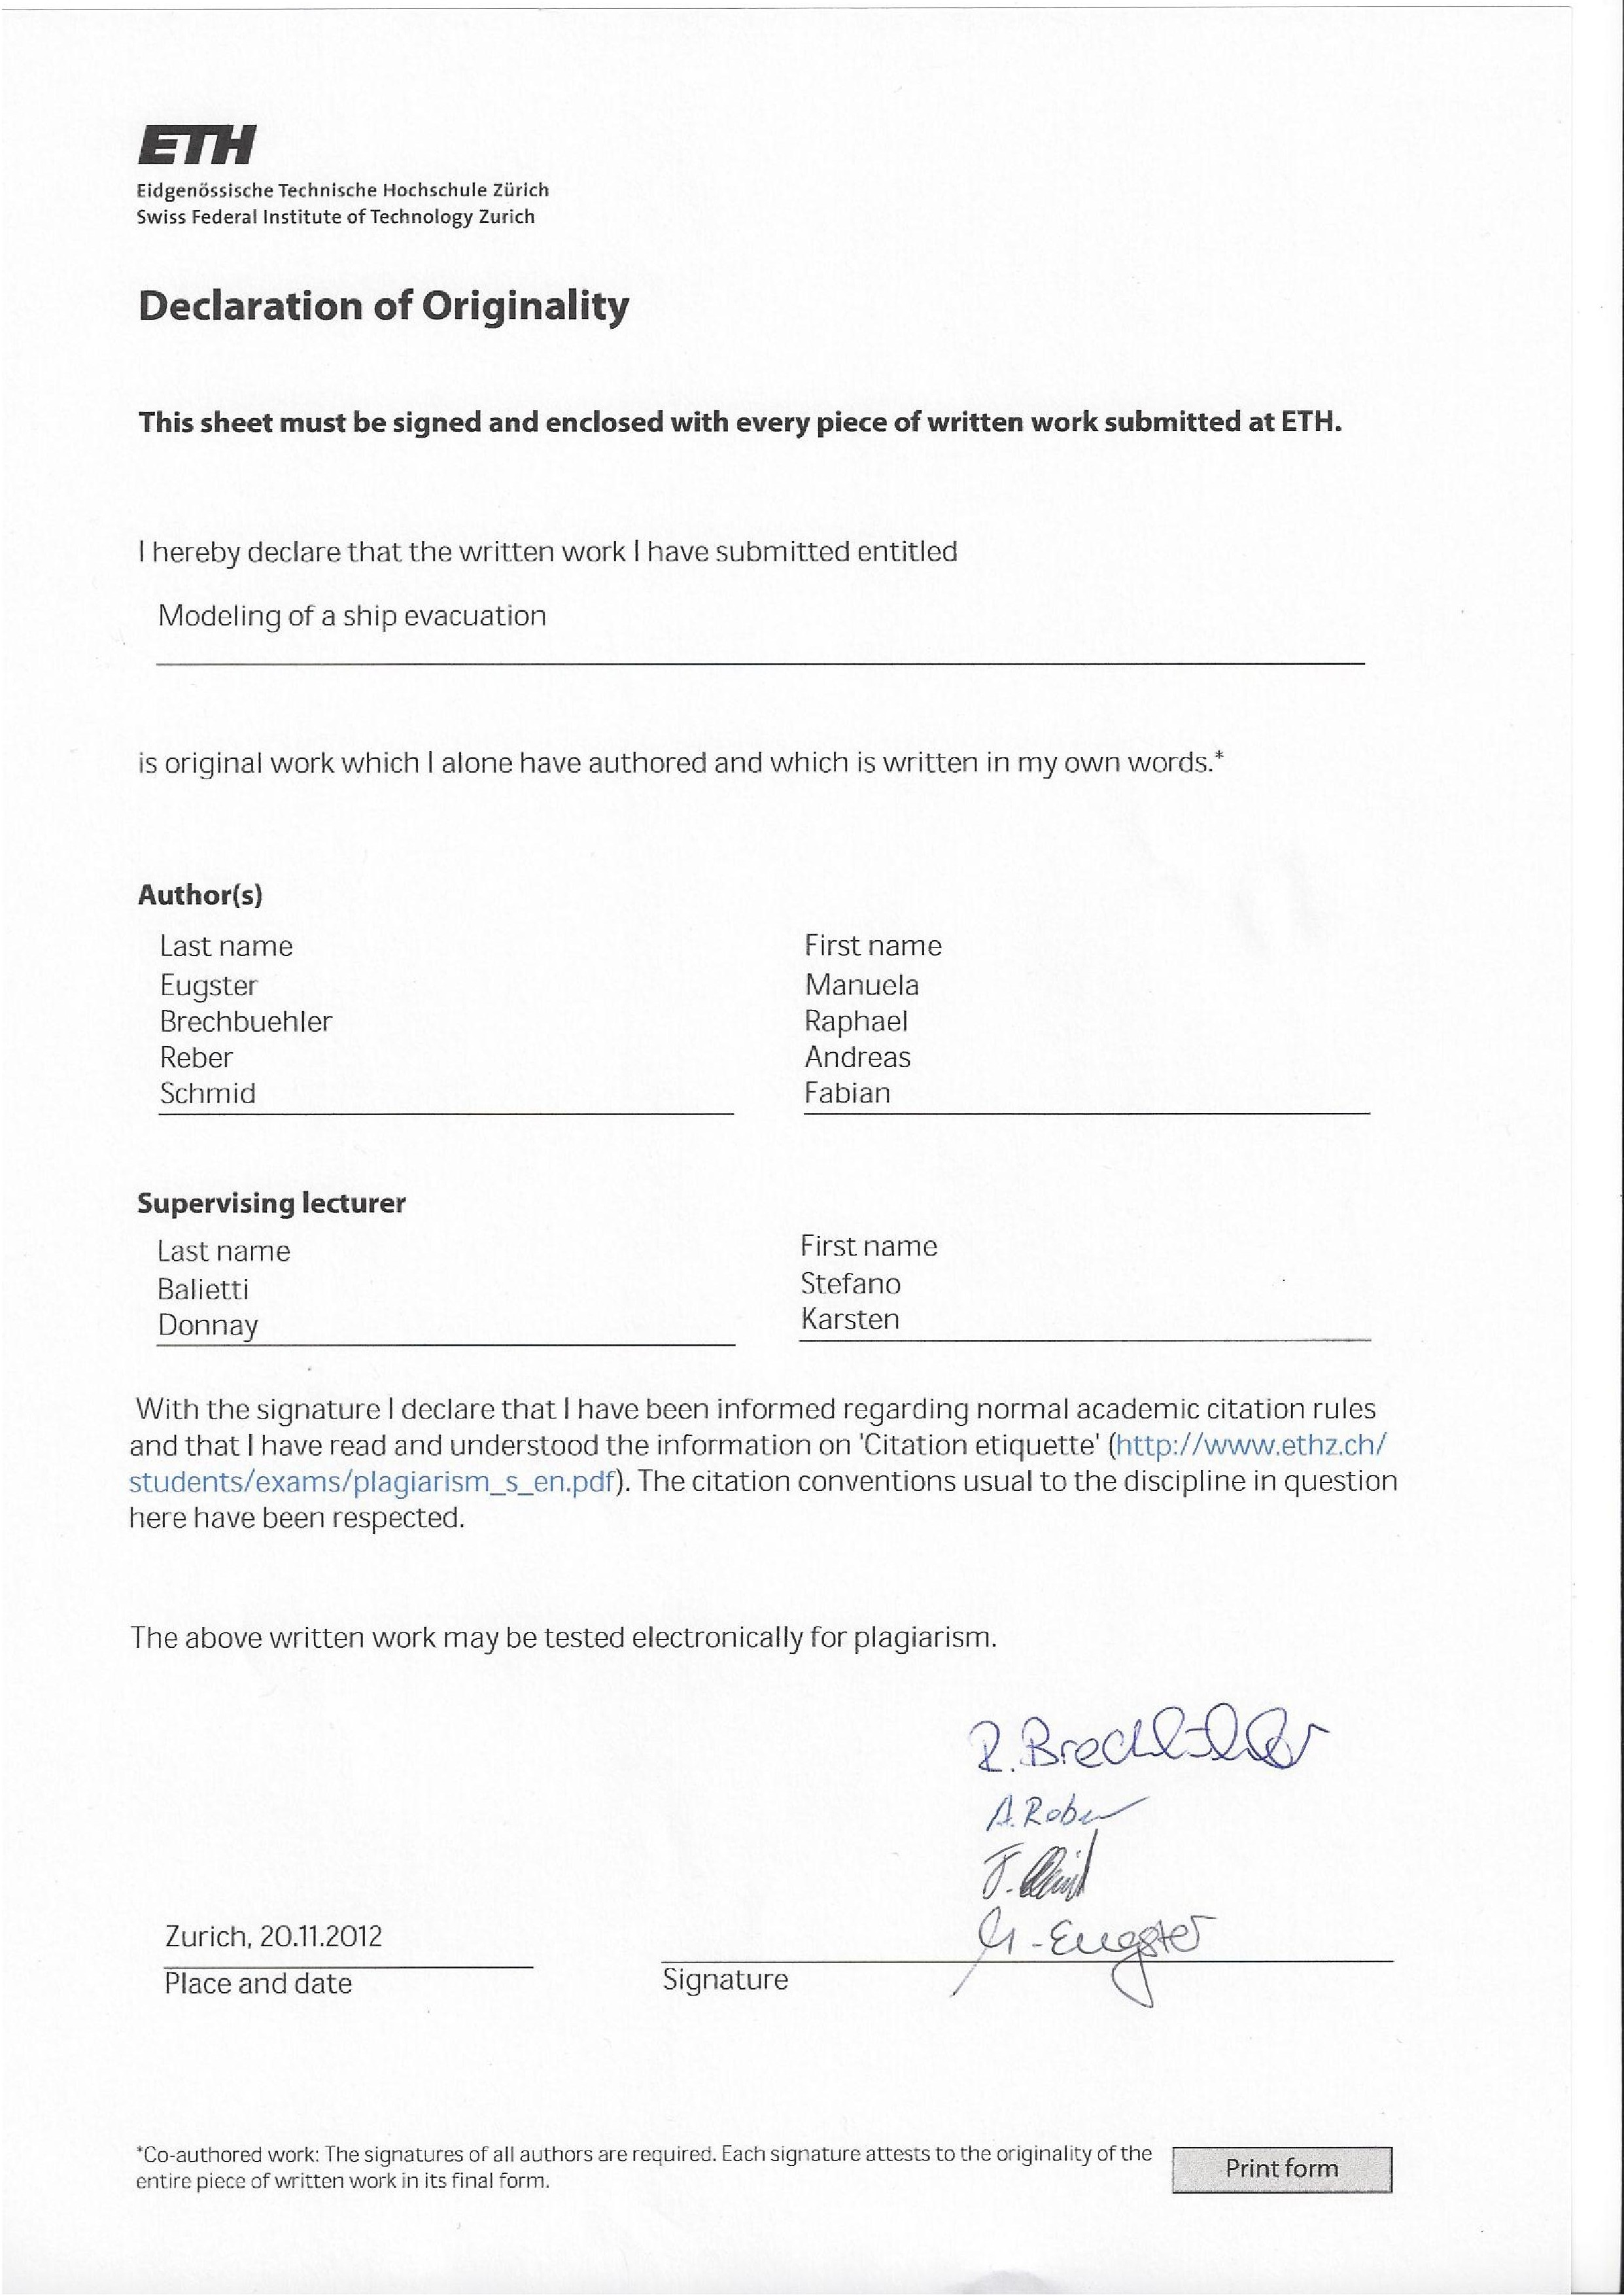
\includegraphics[width=\textwidth]{declaration.jpg}

% IMPORTANT
% you MUST include the ETH declaration of originality here; it is available for download on the course website or at http://www.ethz.ch/faculty/exams/plagiarism/index_EN; it can be printed as pdf and should be filled out in handwriting


%%%%%%%%%% Table of content %%%%%%%%%%%%%%%%%

\tableofcontents

\newpage

%%%%%%%%%%%%%%%%%%%%%%%%%%%%%%%%%%%%%%%



\section{Abstract}

\section{Individual contributions}
The whole project was completed as a team. For sure we took into consideration all the personal backgrounds and  knowledge. That is the reason why Raphael and Manuela focused on implenting the computer code. Whereas Andreas and Fabian concentrated on providing background information, compared the results with the reality and doing its verification.
\section{Introduction and Motivations}
\subsection{Introduction}
The evacuation of a passenger liner due to fire, sinking or other issues leads to several problems. A large amount of passengers try to safe their lives and get to a rescue boat. Narrow and branched floors, smoke, inflowing water, the absence of illumination, rude passengers and so forth can make the evacuation difficult and reduce the number of survivors.
There are a lot of norms how to minimize the harm of such an evacuation. For example there are rules on the number of rescue boats dependent on the amount of passengers \cite{SOLAS}. With dry runs the staff is prepared for the case of emergency et cetera. In real life ship corridor reproduction, the behavior of distressed people is studied.
Another approach is to model such ship evacuations numerically on the computer. As an example the software maritimeEXODUS by a development team from the University of Greenwich is a PC based evacuation and pedestrian dynamics model that is capable of simulating individual people, behaviour and vessel details. The model includes aspects of people-people, people-structure and people-environment interaction. It is capable of simulating thousands of people in very large ship geometries and can incorporate interaction with fire hazard data such as smoke, heat and toxic gases and angle of heel” \cite{EXODUS}.
Our approach is similarly to model a passenger ship with a common geometrical outline and ground view. In an optimization process we will thereafter look for an ideal ground view, rescue boat distribution and their size to minimize the time needed for evacuation. Finally we will make a statement on possible improvements.
\newpage
\subsection{Motivation}
Even though modern ocean liners are considered to be safe, the latest occasions attested that there is still potential for evacuation and safety improvements \cite{concordia}. Certainly we know that this science is very advanced and practised since the sinking of the Titanic. Nevertheless knowing that there are still bottlenecks on the ships we are very motivated to detect and eliminate them with our mathematical models.

\subsection{Fundamental Questions}
To find these bottlenecks we run a mathematical model of a ship structure  with several decks and its passengers \cite{shipdecks}. After we localised these places we are interested in the answers of the folowing questions:

\bigskip
How much time can be saved by varying the dependent variables mentioned below:
\begin{itemize}
\item How much people can be saved by changing the disposition of the specific room types?
\item Where are the bottlenecks during the evacuation? How can they be avoided?
\end{itemize}

What is the influence of the rescue boats?
\begin{itemize}
\item Are small or bigger boats better?
\item Where do they have to be positioned?
\end{itemize}

If we have time to spare we analyse the difference between uncontrolled and controlled passenger flow:
\begin{itemize}
\item Is the crew able to prevent chaos in the evacuation process?
\item What is the best way to lead the passengers out of the ship?
\end{itemize}

In addition we are keen to know if our model is a good abstraction of the reality?

\section{Description of the Model}
\subsection{General Model}

We will base the modeling part on the work done by a group of former "MSSSM" students, by name Hans Hardmeier, Andrin Jenal , Beat Kueng and Felix Thaler. \cite{Building} In their work "Modeling Situations of Evacuation in a Multi-level Building" they wrote a computer program in c with a MATLAB surface to rapidly simulate the evacuation of multi-level buildings.\bigskip

Similar to the building we necessarily need an  implementation of a common ship shape \cite{shipdecks}. In order to make strong conclusions we want to keep the following variables independent:
\begin{itemize}
\item Number of passengers (4400 agents)
\item Overall capacity of the rescue boats (4680 seats)
\item Ship size and shape
\item Area used by specific rooms (coaches for passengers, lounge area, corridors)
\end{itemize}
Our target is to decrease the evacuation time. Measurements will be made on the time to evacuate:
\begin{itemize}
\item 10\%
\item 50\%
\item 90\%
\item100\% of all passengers.
\end{itemize}
In order to optimize the evacuation time, we change the following dependent variables:
\begin{itemize}
\item Disposition of the specific room types (e.g. changing the geometry of the corridors without changing the total area used for corridors)
\item Rescue boat size, number and position
\item Control of the passenger flow by crew members (e.g. is there staff to lead the passengers and how are they doing it?)
\end{itemize}




\section{Implementation}
\subsection{Code}
\subsection{Ship Decks}
\section{Simulation Results and Discussion}
\subsection{Expected Results}
\begin{itemize}
\item Even though modern ships are quite optimized in regard to evacuation time, they are always a compromise between safety and luxury. Therefore we are convinced to find a superior adjustment of the decks geometries to increase the survival rate.
\item Since the rescue boats can not be averaged but are rather concentrated over one or two decks, we consider the staircases as the bottlenecks.
\item In alinging this variables we are persuaded of a reduction of the overall evacuation time.
\item We suppose that smaller and evenly spread rescue boats combined with a higher quantity will scale the evacuation time down. Certainly there is going to be an optimum in size which we are willing to find.
\item By controlling the rescue we assume to detect a huge decrease in evacuation time. Further we have the hypothesis that disorder can be minimized. The crew who is familiar with the decks and the emergency exits is able to guide the passengers in minimum time to the rescue boats.
\item There are many parameters we do not model in our simulation. For example fire and smoke, the tilt of the ship or handicapped and petrified passengers are disregarded. By leaving out this details we get a very simplified model. However, by starting the optimization process by data of a nowadays passenger liner \cite{shipdecks} we hope to see some real evacuation dynamics in this system and therefore make conclusion on the fundamental questions.
\end{itemize}
\subsection{Simulation Results}
\subsubsection{Standard ship}
As listed above we were interested in the time in which a certain percentage of all agents was evacuated:
\newline

\begin{figure}
\centering
\begin{tabular}
{|>{\large}m{2cm} |>{\center}b{1.1cm} |>{\center}b{1.1cm}|>{}b{1.1cm}|>{}b{1.1cm}|} \hline \hline
percantage of agents.& 10\% &  50\% & 90\% &100\% \\ \hline
evacuation time & 69s &272s & 468s & 694s \\ \hline \hline
\end{tabular}
\caption{Needed time to evacuate a certain percentage of all agents.}
\end{figure}

Further our standard ship simulation 

\subsubsection{Modified rescueboat size}
\subsubsection{Modified room disposition}
\subsubsection{Merge of modified room disposition and rescueboat size}
\subsection{Comparison}
\subsection{Discussion}
\section{Summary and Outlook}
\subsection{Summary}
\subsection{Outlook}
\section{References}

\begin{thebibliography}{9}
\bibitem{Helbling} Helbing, Dirk (1995): Social Force Model for Pedestrians Dynamics.
\bibitem{Building} Hardmeier,Jenal,Kueng,Thaler (2012): Modelling Situations of Evacuation in a Multi-level Building.
\bibitem{SOLAS} SOLAS (1974): International Convention for the Safety of Life at Sea. \url{http://www.imo.org/about/conventions/listofconventions/pages/international-convention-for-the-safety-of-life-at-sea-(solas),-1974.aspx}
\bibitem{ship} SHIP EVACUATION: \url{http://www.shipevacuation.com/}
\bibitem{shipdecks} CRUISE DECK PLANS PUBLIC SITE: \url{http://www.cruisedeckplans.com/DP/Main/decks.php?ship=Costa%20Serena}
\bibitem{EXODUS} University of Greenwich (2011):  maritimeEXODUS. \url{http://fseg.gre.ac.uk/fire/marine_evac_model.html}
\bibitem{concordia} Haverie of Costa Concordia (2012): \url{http://de.wikipedia.org/wiki/Costa_Concordia#Havarie_2012}
	
\end{thebibliography}

\end{document}  

 
